\subsection{Strømforsyning}

For at frigøre sig fra laboratoriets strømforsyningerne udarbejdes egen strømforsyning. Vha en 230Vac/12Vdc transformerer og egnede spændingens,-regulatorer og delere designes en strømforsyning til netop dette projekt. Masteren (DevKit8000) har sin egen strømforsyning og denne ændres ikke. Enheden (PSoC4) skal forsynes med 5V dc via USB. Relæstyringen skal forsynes med 5V dc. PIR sensoren skal forsynes med 5-20 V dc. Temperatur/fugt sensoren skal forsynes med 3,3V dc. 

230Vac/12Vdc transformeren er fra en gammel computer. Denne kan give 2 amperre og er forsynet med et DC stik (12V) og en stikprop (230Vac). Denne transformer bruges som den er. 

For at regulere fra de 12 V til 5 V benyttes en spændingsregulator. LM7805 er beregnet netop til dette formål. Ud fra databladet (Side 2/19 LM7805.pdf) Ses forbindelsen af LM7805'ern.

\begin{figure}[H] \centering
{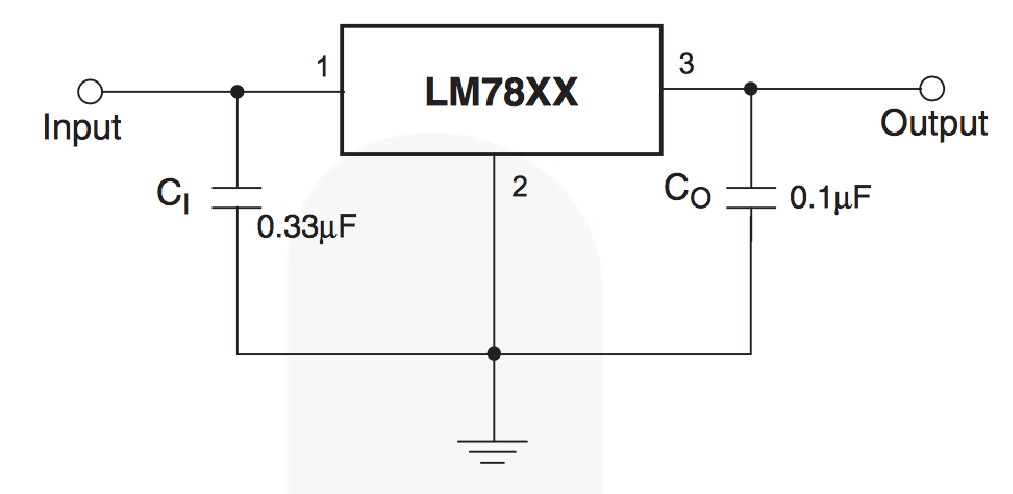
\includegraphics[width=\textwidth]{filer/design/Billeder/LM7805_DATASHEET}}
\caption{Forbindelse af LM7805 - Side 2/19 LM7805.pdf}
\label{lab:LM7805}
\raggedright
\end{figure}

Spændingsregulatoren LM7805 er opbygget i mutilsim, sammen med 12V dc forsyningen. Kredløbet er simuleret og dette viser at outputtet er de ønskede 5 V.

\begin{figure}[H] \centering
{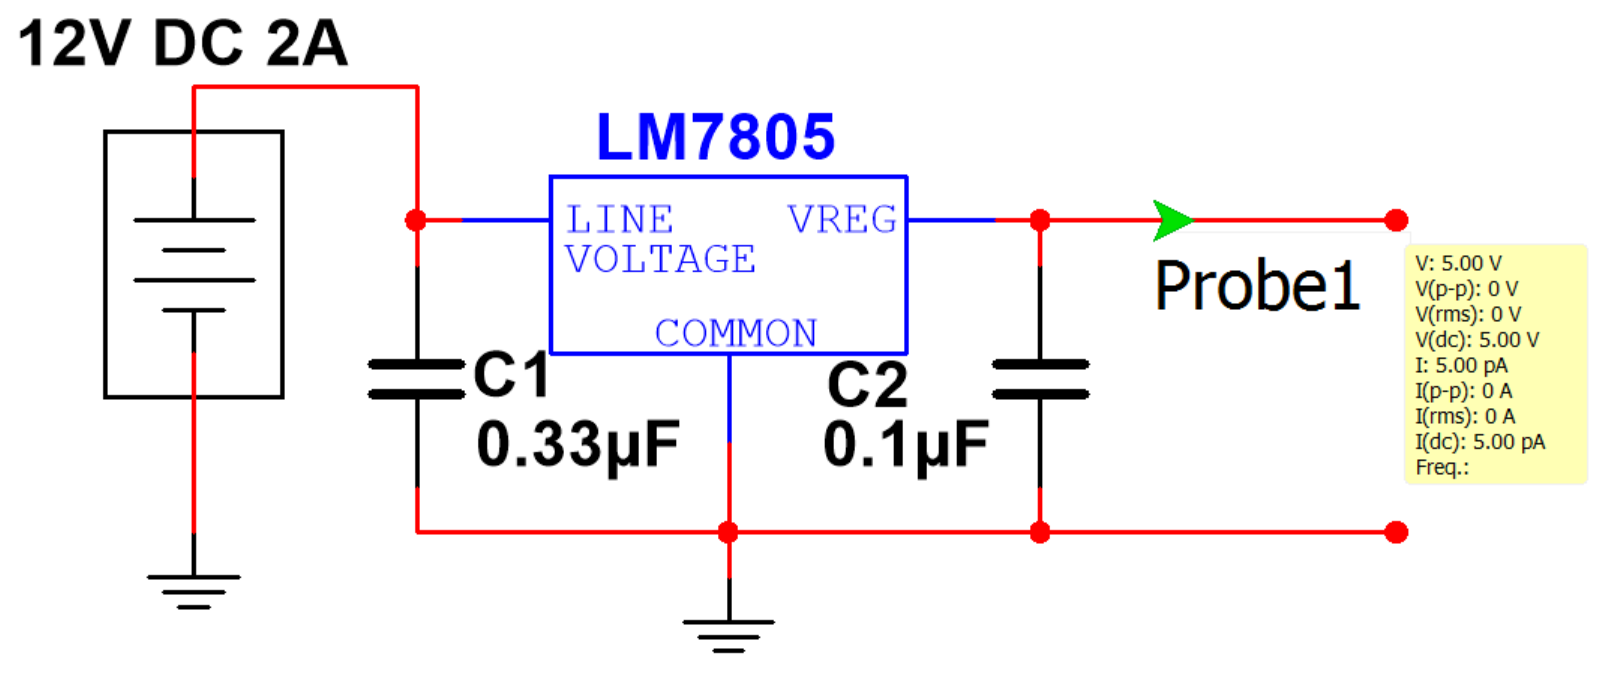
\includegraphics[width=\textwidth]{filer/design/Billeder/LM7805_SIMULATION}}
\caption{LM7805 Simulering}
\label{lab:LM7805_SIMULERING}
\raggedright
\end{figure}

------
En løsning 1k ohm?  - en spændingsregulator er nok at foretrække?
Skal byttes ud med LM317
------

For at opnå de 3,3V opbygges en spændings deler. 3,3 V er netop 2/3 af 5 V. Herved sættes 3 ens modstande i serie. Herved vil spændingen være ens over alle modstande. 5 V i den ene ende af serien og 0 V ground i den anden, vil der opnås 2 punkter, et med 3,3 V og et med 1,65 V. Spændingsdeleren er opbygget i multisim og simuleringen viser de ønskede 3.3 V

 
\begin{figure}[H] \centering
{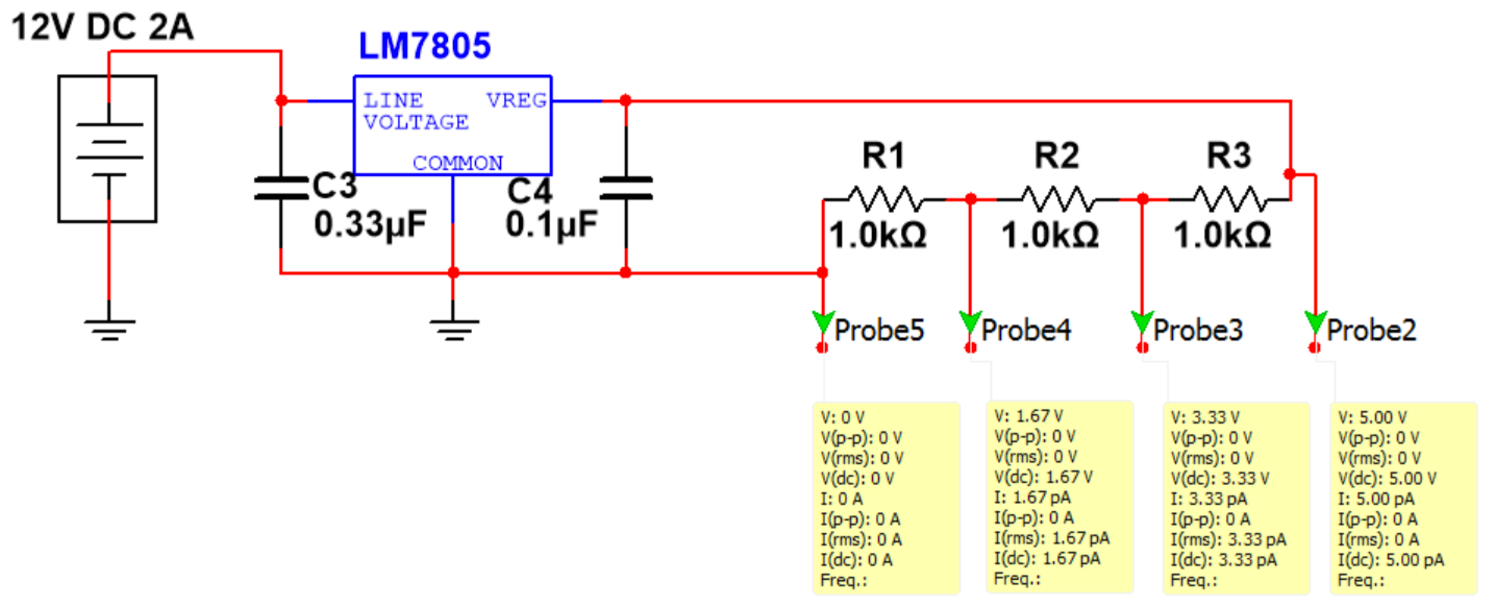
\includegraphics[width=\textwidth]{filer/design/Billeder/33V_SIMULATION}}
\caption{Simulering af 3.3 V vha. spændingsdeler}
\label{lab:3.3V_SIMULERING}
\raggedright
\end{figure}

Næste step er at føre hhv. 5 V og 3.3 V til de rigtige steder. Dette gøres vha. et tilslutnignsprint

\subsection{Tilslutningsprint}

Tilslutningsprintet sørger for at sammenkoble Enheden med de ønskede sensorer, samt at forsyne Enhed og sensorer med ønsket forsyning.